
\documentclass{article}

%\usepackage[utf8]{inputenc}
%\usepackage[a4paper, total={7in, 8in}]{geometry}
\usepackage[left=15mm,top=26mm,right=8mm,bottom=15mm]{geometry}

\usepackage{spverbatim}
\usepackage{minted}
\usepackage{amssymb}
\usepackage{bm}
\usepackage{graphicx}
\usepackage{amsmath}
\usepackage{enumerate}
%\setlength{\voffset}{-0.75in}
%\setlength{\headsep}{-10pt}


\title{EECE 5639- Homework 6: Homographies, Stereo and Motion}
\author{Sreejith Sreekumar: 001277209}
\date{\today}
\begin{document}

\maketitle

\section*{Question 1}
Homography is a 2D - 2D projective transformation between the pixel coordinates in two images that one
viewing the same plane from different angles, taken from the camera. In homography, the camera is rotated
about its centre of projection without any translation. In other words, planar homography relates the transformation between two planes. \\

$\begin{bmatrix}
    x'\\
    y'\\
    1'\\
\end{bmatrix}$ = H $\begin{bmatrix}
    x\\
    y\\
    1\\
\end{bmatrix}$ = $\begin{bmatrix}
    h_{11} &  h_{12} &  h_{13}\\
    h_{21} &  h_{22} &  h_{21}\\
    h_{31} &  h_{32} &  h_{33}\\
\end{bmatrix}$ $\begin{bmatrix}
    x\\
    y\\
    1\\
\end{bmatrix}$ \\

In stereo vision, which is the ability to infer information on the 3D structure and distance of a
scene from two or more images taken from different viewpoints, we use Essential and Fundemental matrices to
construct correspondence equations.

The essential matrix is a 3 x 3 matrix that encodes the epipolar geomtry of two views. Given a point
in an image, multiplying by the Essential Matrix, will tell us the epipolar line in the second image
where the corresponding point must be.
If $P_{l}$ and $P_{r}$ are two two points from the left and right cameras of the stereo, we have:
\[
P_{r}^{T} R.S P_{l} = 0
\]
Where R is the rotation matrix and S is the matrix which depends on the baseline translation. Using the
Longuet Higgins equation we also have
\[
p_{r}^{T} R.S p_{l} = 0
\]
where $p_{l}$ and $p_{r}$ are the camera coordinates. Now adding instrinsic parameters to this equation,
we have an equation of the form:

\[
\overline{p_{r}}^{T} ( M_{r}^{-T}EM_{l}^{-T})\overline{p_{l}} = 0
\]
or 
\[
\overline{p_{r}}^{T} F \overline{p_{l}} = 0
\]
F, The fundemental matrix here is analogous to the Essential matrix, and tells how points in
each image are related to epipolar lines in the other image. It depends on the extrinsic and intrinsic
parameters. \\

\section*{Question 2}
Epipoles in the canonical configuration will be at infinity.

\section*{Question 3}
Planar Affine Camera Model \\

\begin{itemize}
  
\item $\begin{bmatrix}
    su\\
    sv\\
    s\\
\end{bmatrix}$ $\begin{bmatrix}
    p_{11} &  p_{12} &  p_{13}\\
    p_{21} &  p_{22} &  p_{23}\\
    0 &  0 &  p_{33}\\
\end{bmatrix}$ $\begin{bmatrix}
    X\\
    Y\\
    1\\
\end{bmatrix}$ \\

Since the scale doesn't matter, \\

$\begin{bmatrix}
    u\\
    v
\end{bmatrix}$ $\begin{bmatrix}
    p_{11} &  p_{12} &  p_{13}\\
    p_{21} &  p_{22} &  p_{21}\\
\end{bmatrix}$ $\begin{bmatrix}
    X\\
    Y\\
    1\\
\end{bmatrix}$ \\

\item If the field of view is such that all points on the world plane have approximately same depth
  from the camera compared to the distance of the camera from plane.

\item Since we have 6 degrees of freedom, we need 3 points.
  
\item Planar affine transformation preserves the parallel property of parallel lines.  
\end{itemize}

\pagebreak
\begin{figure}
  \section*{Question 4}

 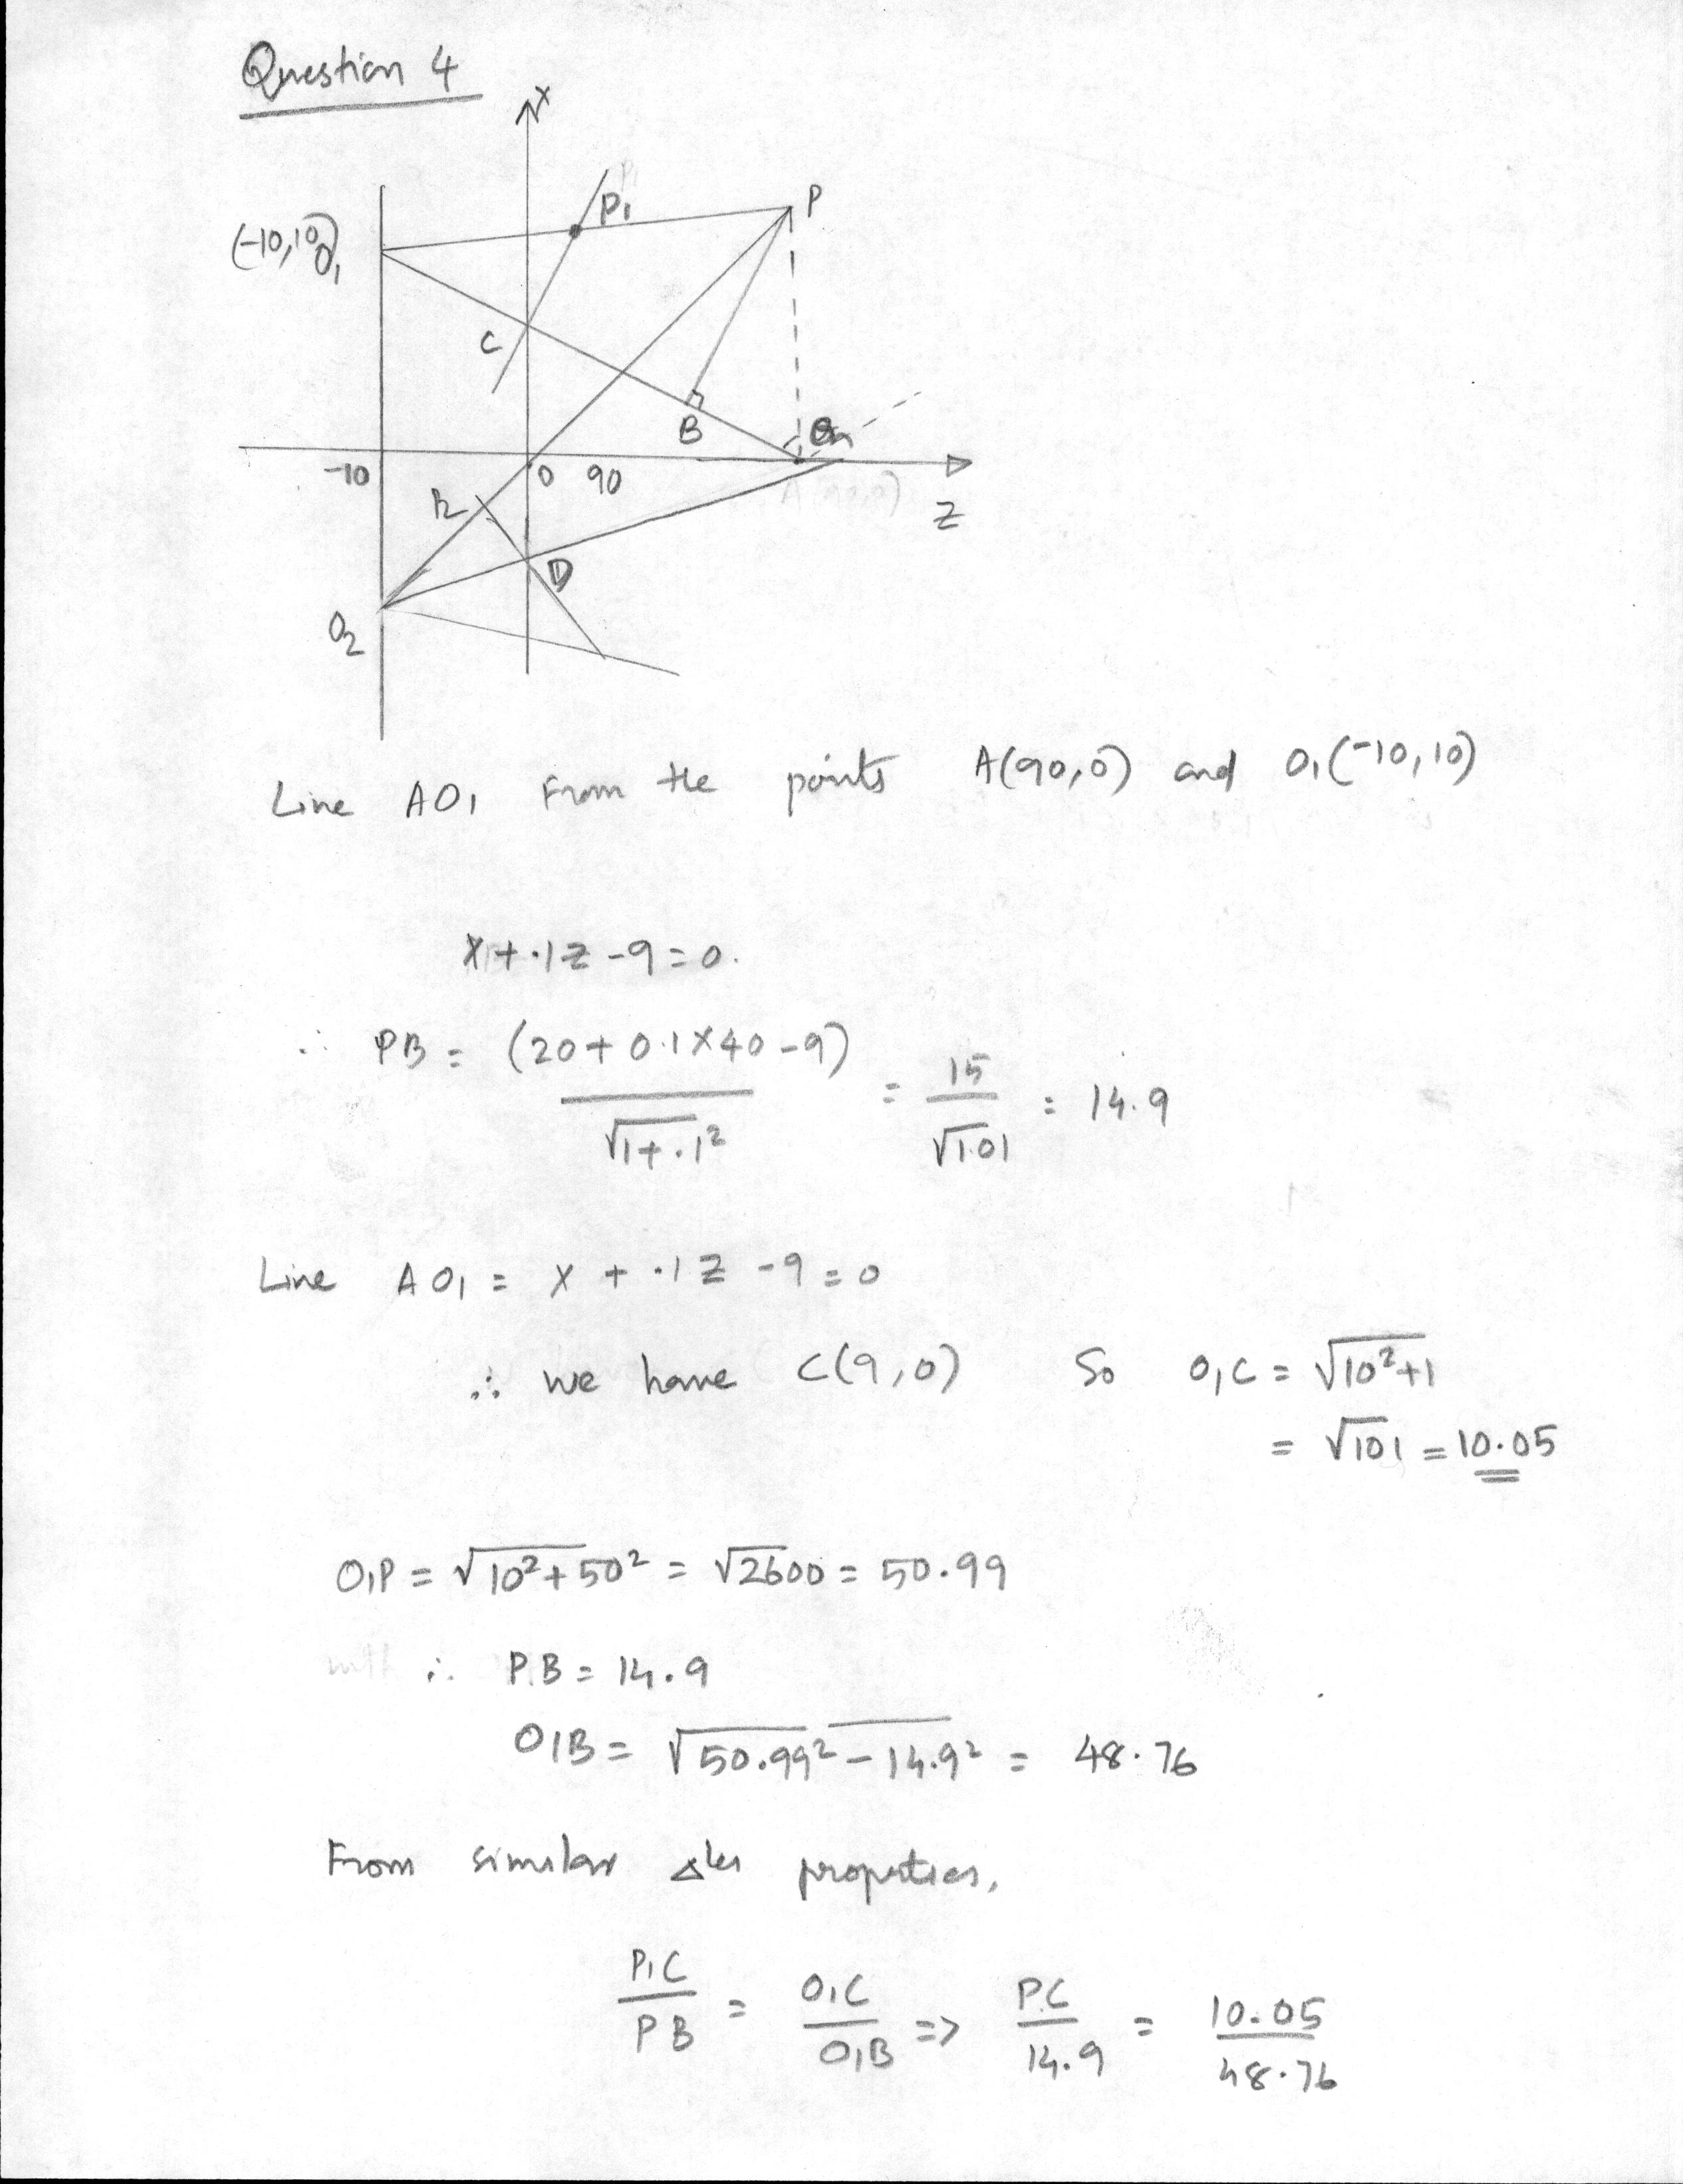
\includegraphics[width=15cm]{1.jpg}
\end{figure}

\pagebreak

\begin{figure}
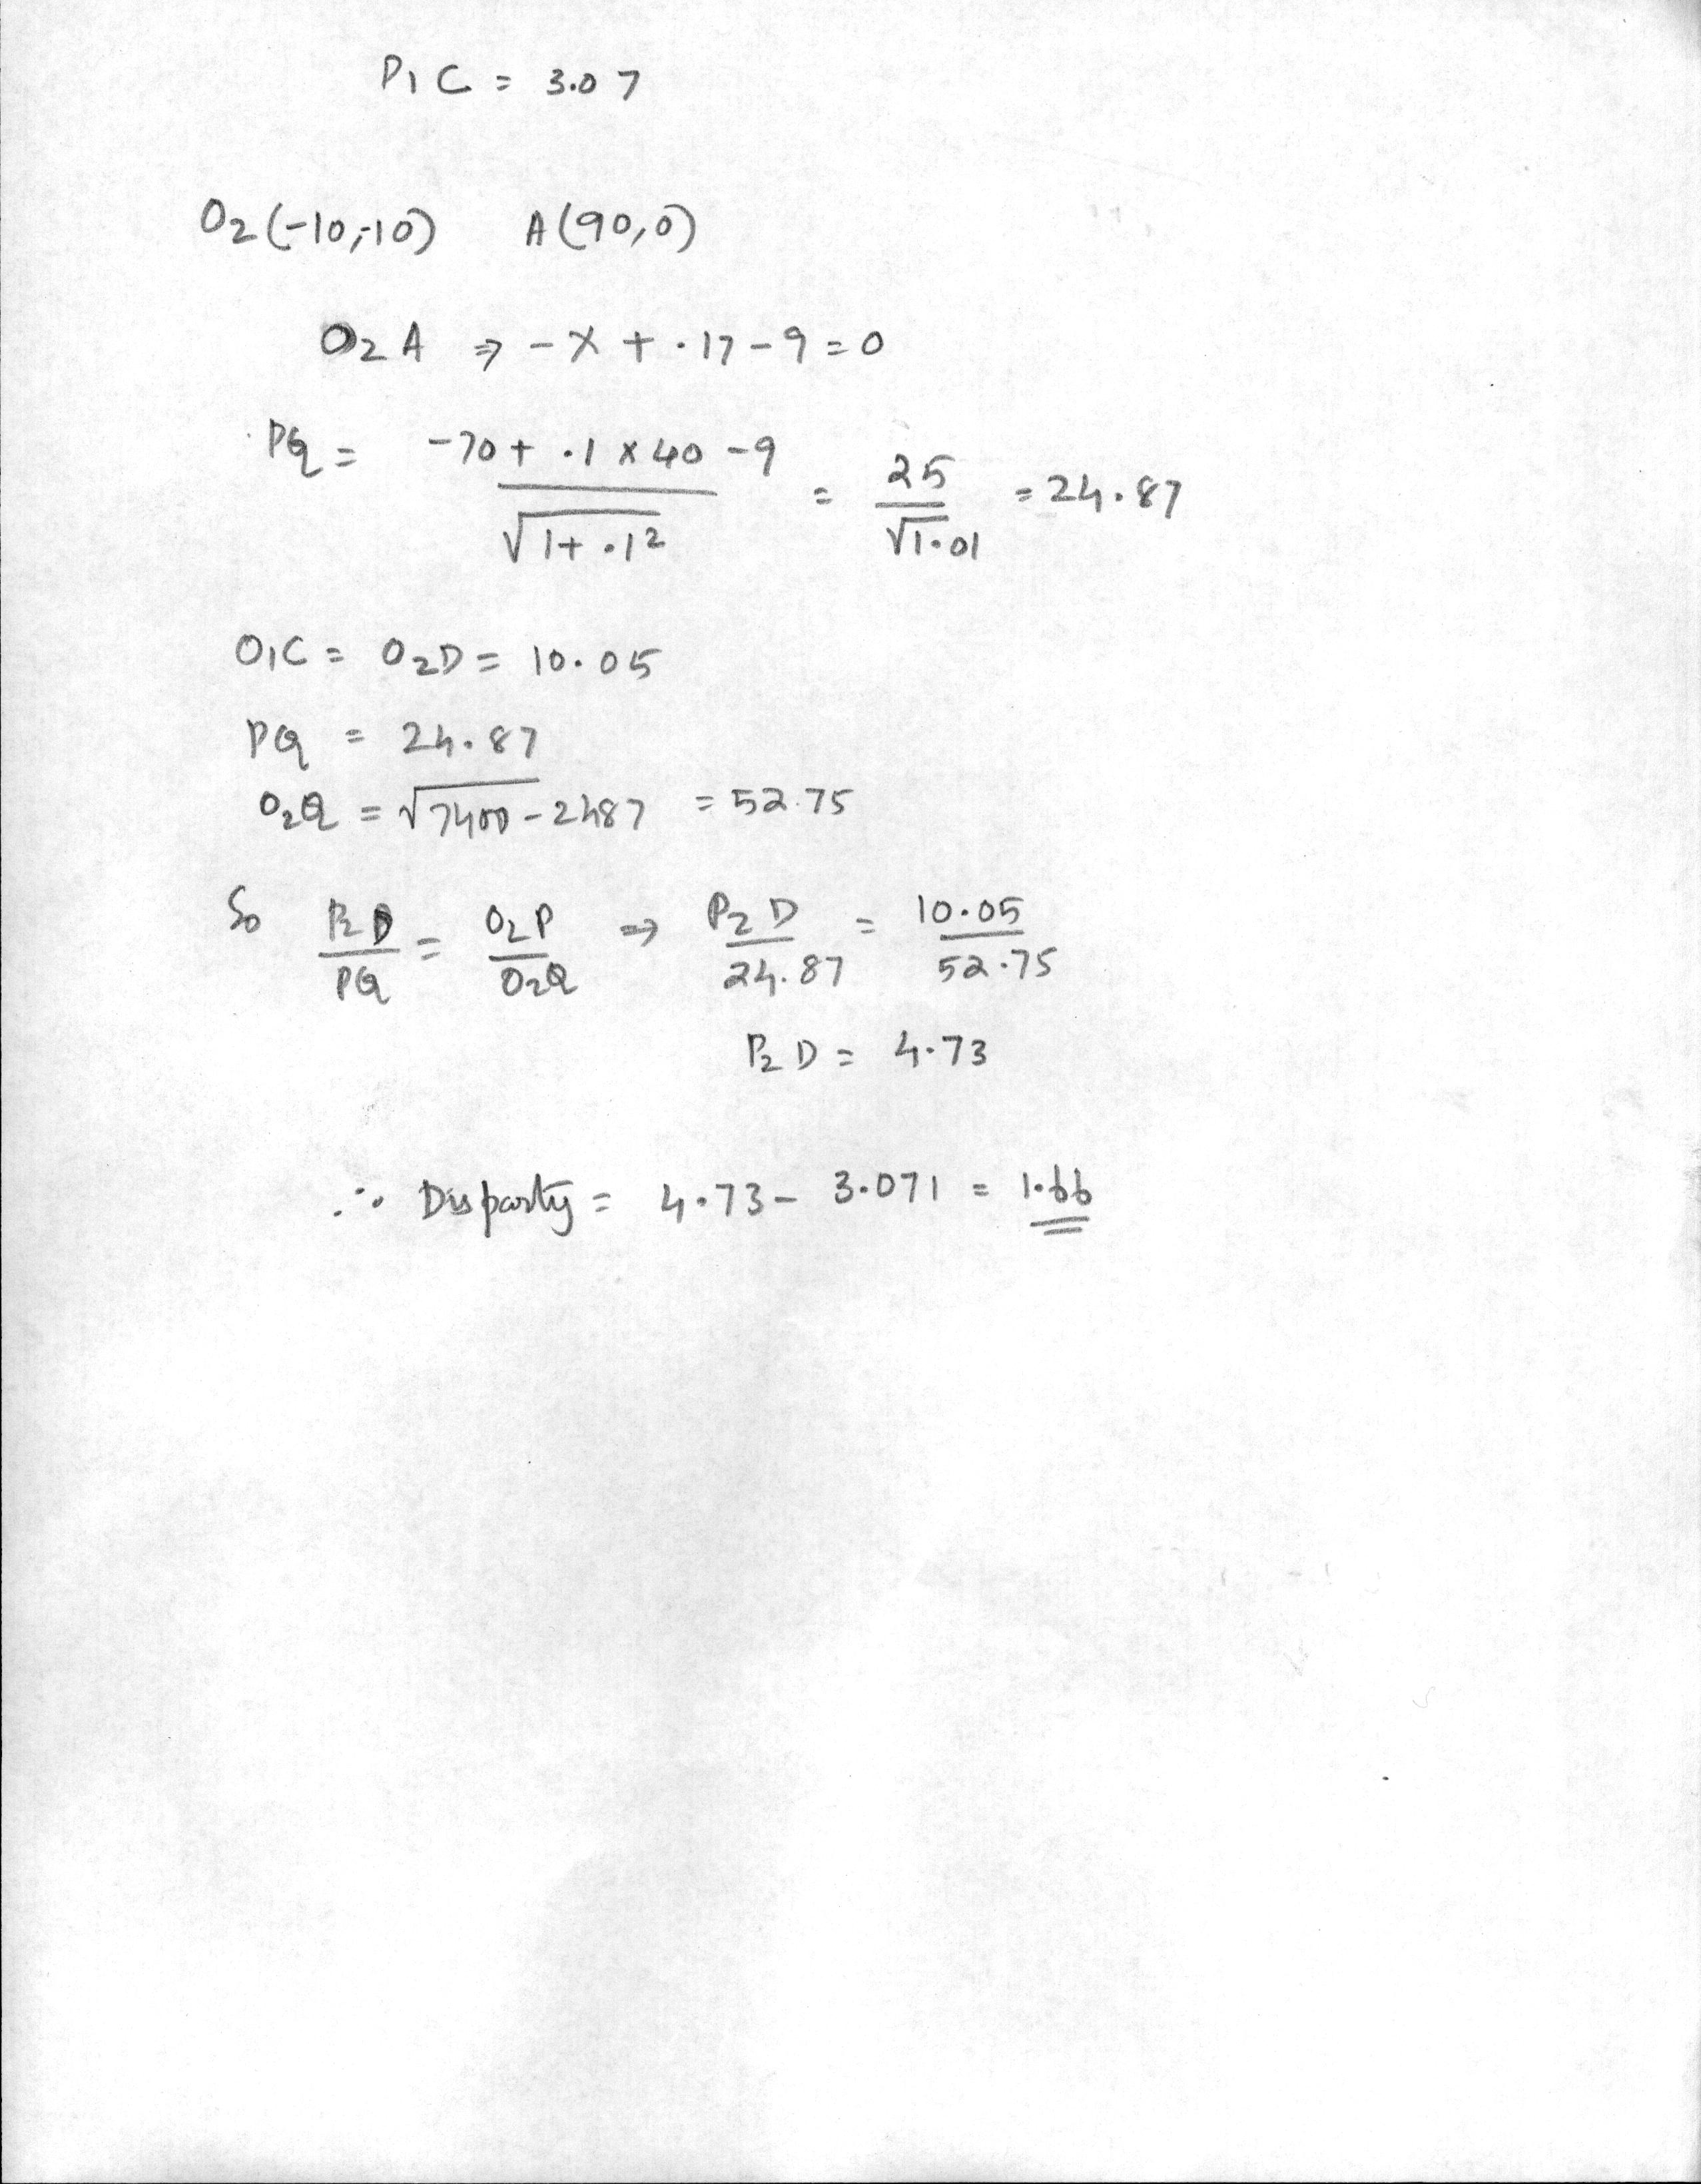
\includegraphics[width=15cm]{2.jpg}
\end{figure}



\textit{Note: Question 4 (scanned page) has been put below Question 5}

\section*{Question 5}



Normalizing the entries of the fundemental matrix: \\

Let the set of points be defined by \\

\[
p_{i} = \begin{bmatrix}
    x_{i}\\
    y_{i}\\
    1\\
\end{bmatrix}^{T}
\]
Now, 
\[
 \overline{x} = \frac{1}{n}\sum_{i}x_{i}\  and\   \overline{y} = \frac{1}{n}\sum_{i}y_{i}
 \]
 where
 \[
 \overline{d} = \frac{\sum_{i}\sqrt{(x_{i} - \overline{x})^{2} + (y_{i} - \overline{y})^{2}}}{n\sqrt{2}}
 \]

 \[
 H\textbf{p} = \hat{p_{i}}
 \]

 i.e,
 \[
\begin{bmatrix}
    h_{11} &  h_{12} &  h_{13}\\
    h_{21} &  h_{22} &  h_{21}\\
    h_{31} &  h_{32} &  h_{33}\\
\end{bmatrix} \begin{bmatrix}
    x_{i}\\
    y_{i}\\
    1\\
\end{bmatrix} = \begin{bmatrix}
    \frac{x_{i} - \overline{x}}{d}\\
    \frac{y_{i} - \overline{y}}{d}\\
    1\\
\end{bmatrix}
\]

\begin{equation}
h_{11}x_{i}  + h_{12}y_{i} +  h_{13} =     \frac{x_{i} - \overline{x}}{d}
\end{equation}
\begin{equation}
h_{21}x_{i}  + h_{22}y_{i} +  h_{23} =     \frac{y_{i} - \overline{y}}{d}
\end{equation}
\begin{equation}
h_{31}  + h_{32} +  h_{33} =     1
\end{equation}

Equating with the co-efficients of $x_{i}$ and $y_{i}$ we have: \\

From eq (1) above
$h_{11}x_{i}$ = $\frac{x_{i}}{d}$, 
$h_{12}$ = 0, 
$h_{13} = \frac{\overline{-x}}{d}$ \\

From eq(2)
$h_{21} = 0$,
$h_{22} = \frac{1}{d}$,
$h_{23} = \frac{\overline{y}}{d}$ \\

From (3)
$h_{31} = 0$,
$h_{32} = 0$,
$h_{33} = 1$  \\


Hence, the normalizing matrix is: \\
\[
\begin{bmatrix}
    \frac{1}{d} &  0 &  \frac{\overline{-x}}{d}\\ \\
    0 & \frac{1}{d} &  \frac{\overline{y}}{d}\\ \\
    0 &  0 & 1\\
\end{bmatrix} 
\]


\begin{figure}
\section*{Question 6}
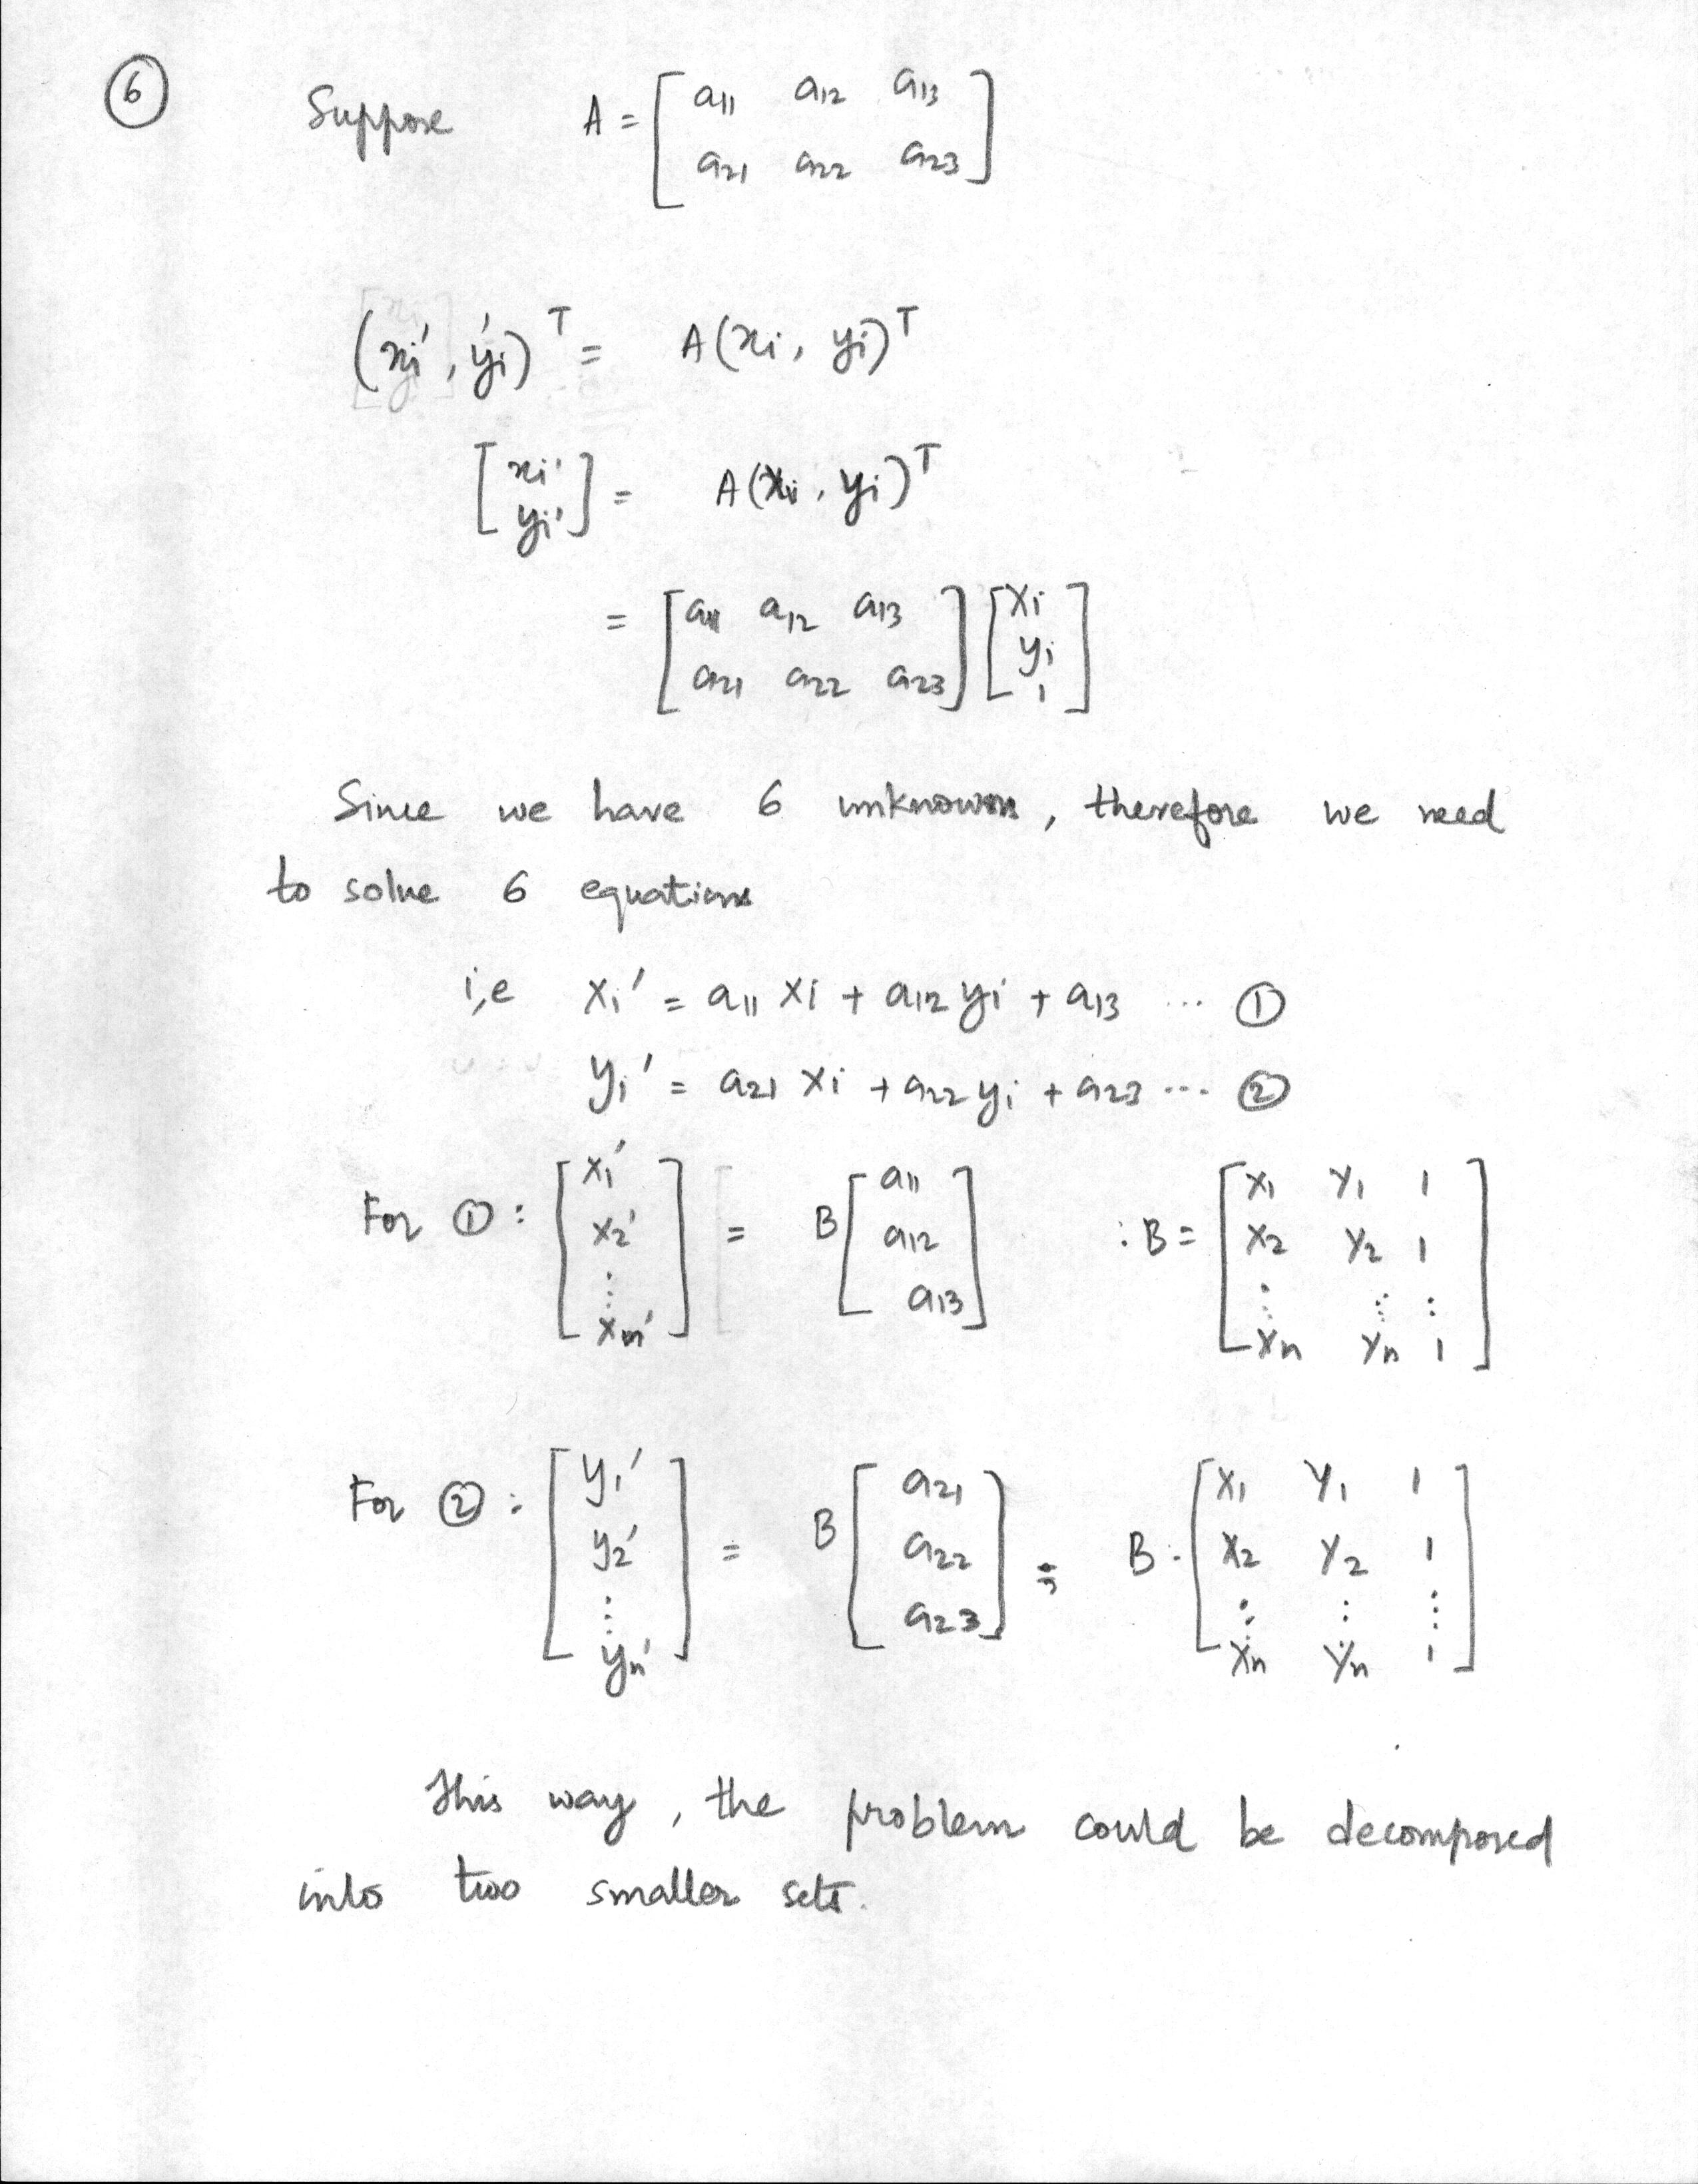
\includegraphics[width=15cm]{3.jpg}
\end{figure}

\begin{figure}
\section*{Question 7}  
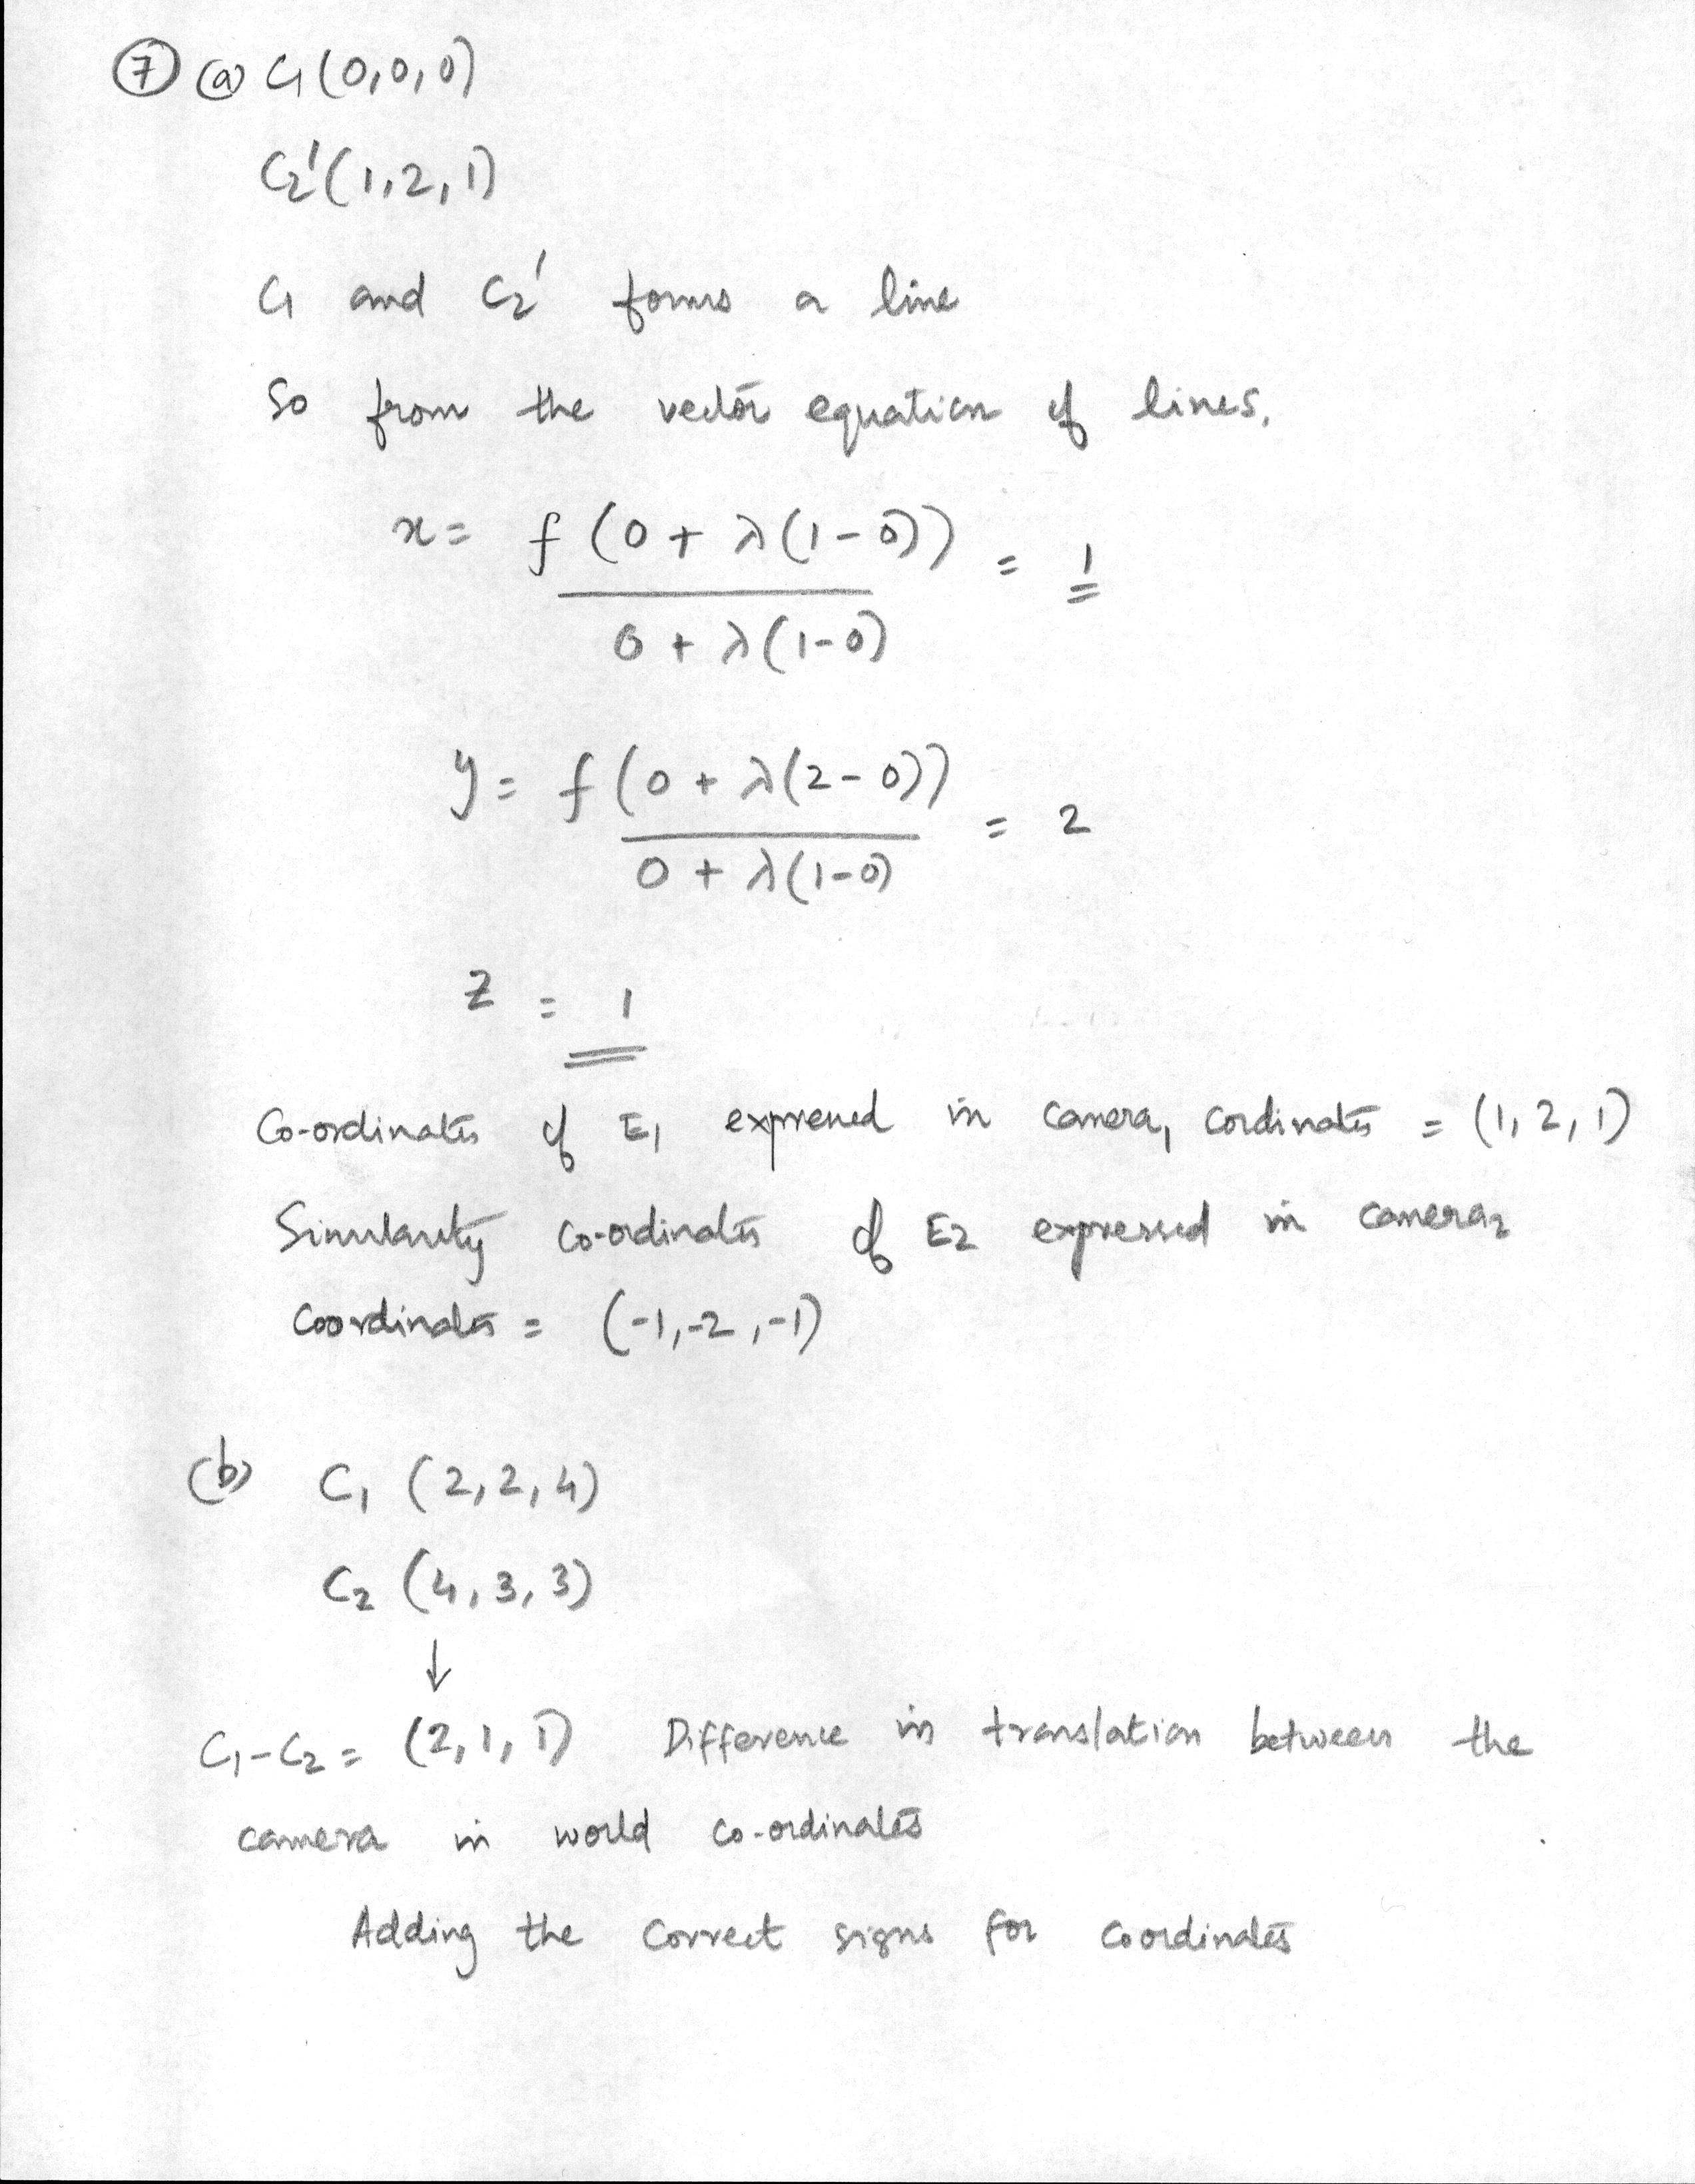
\includegraphics[width=15cm]{4.jpg}
\end{figure}

\begin{figure}
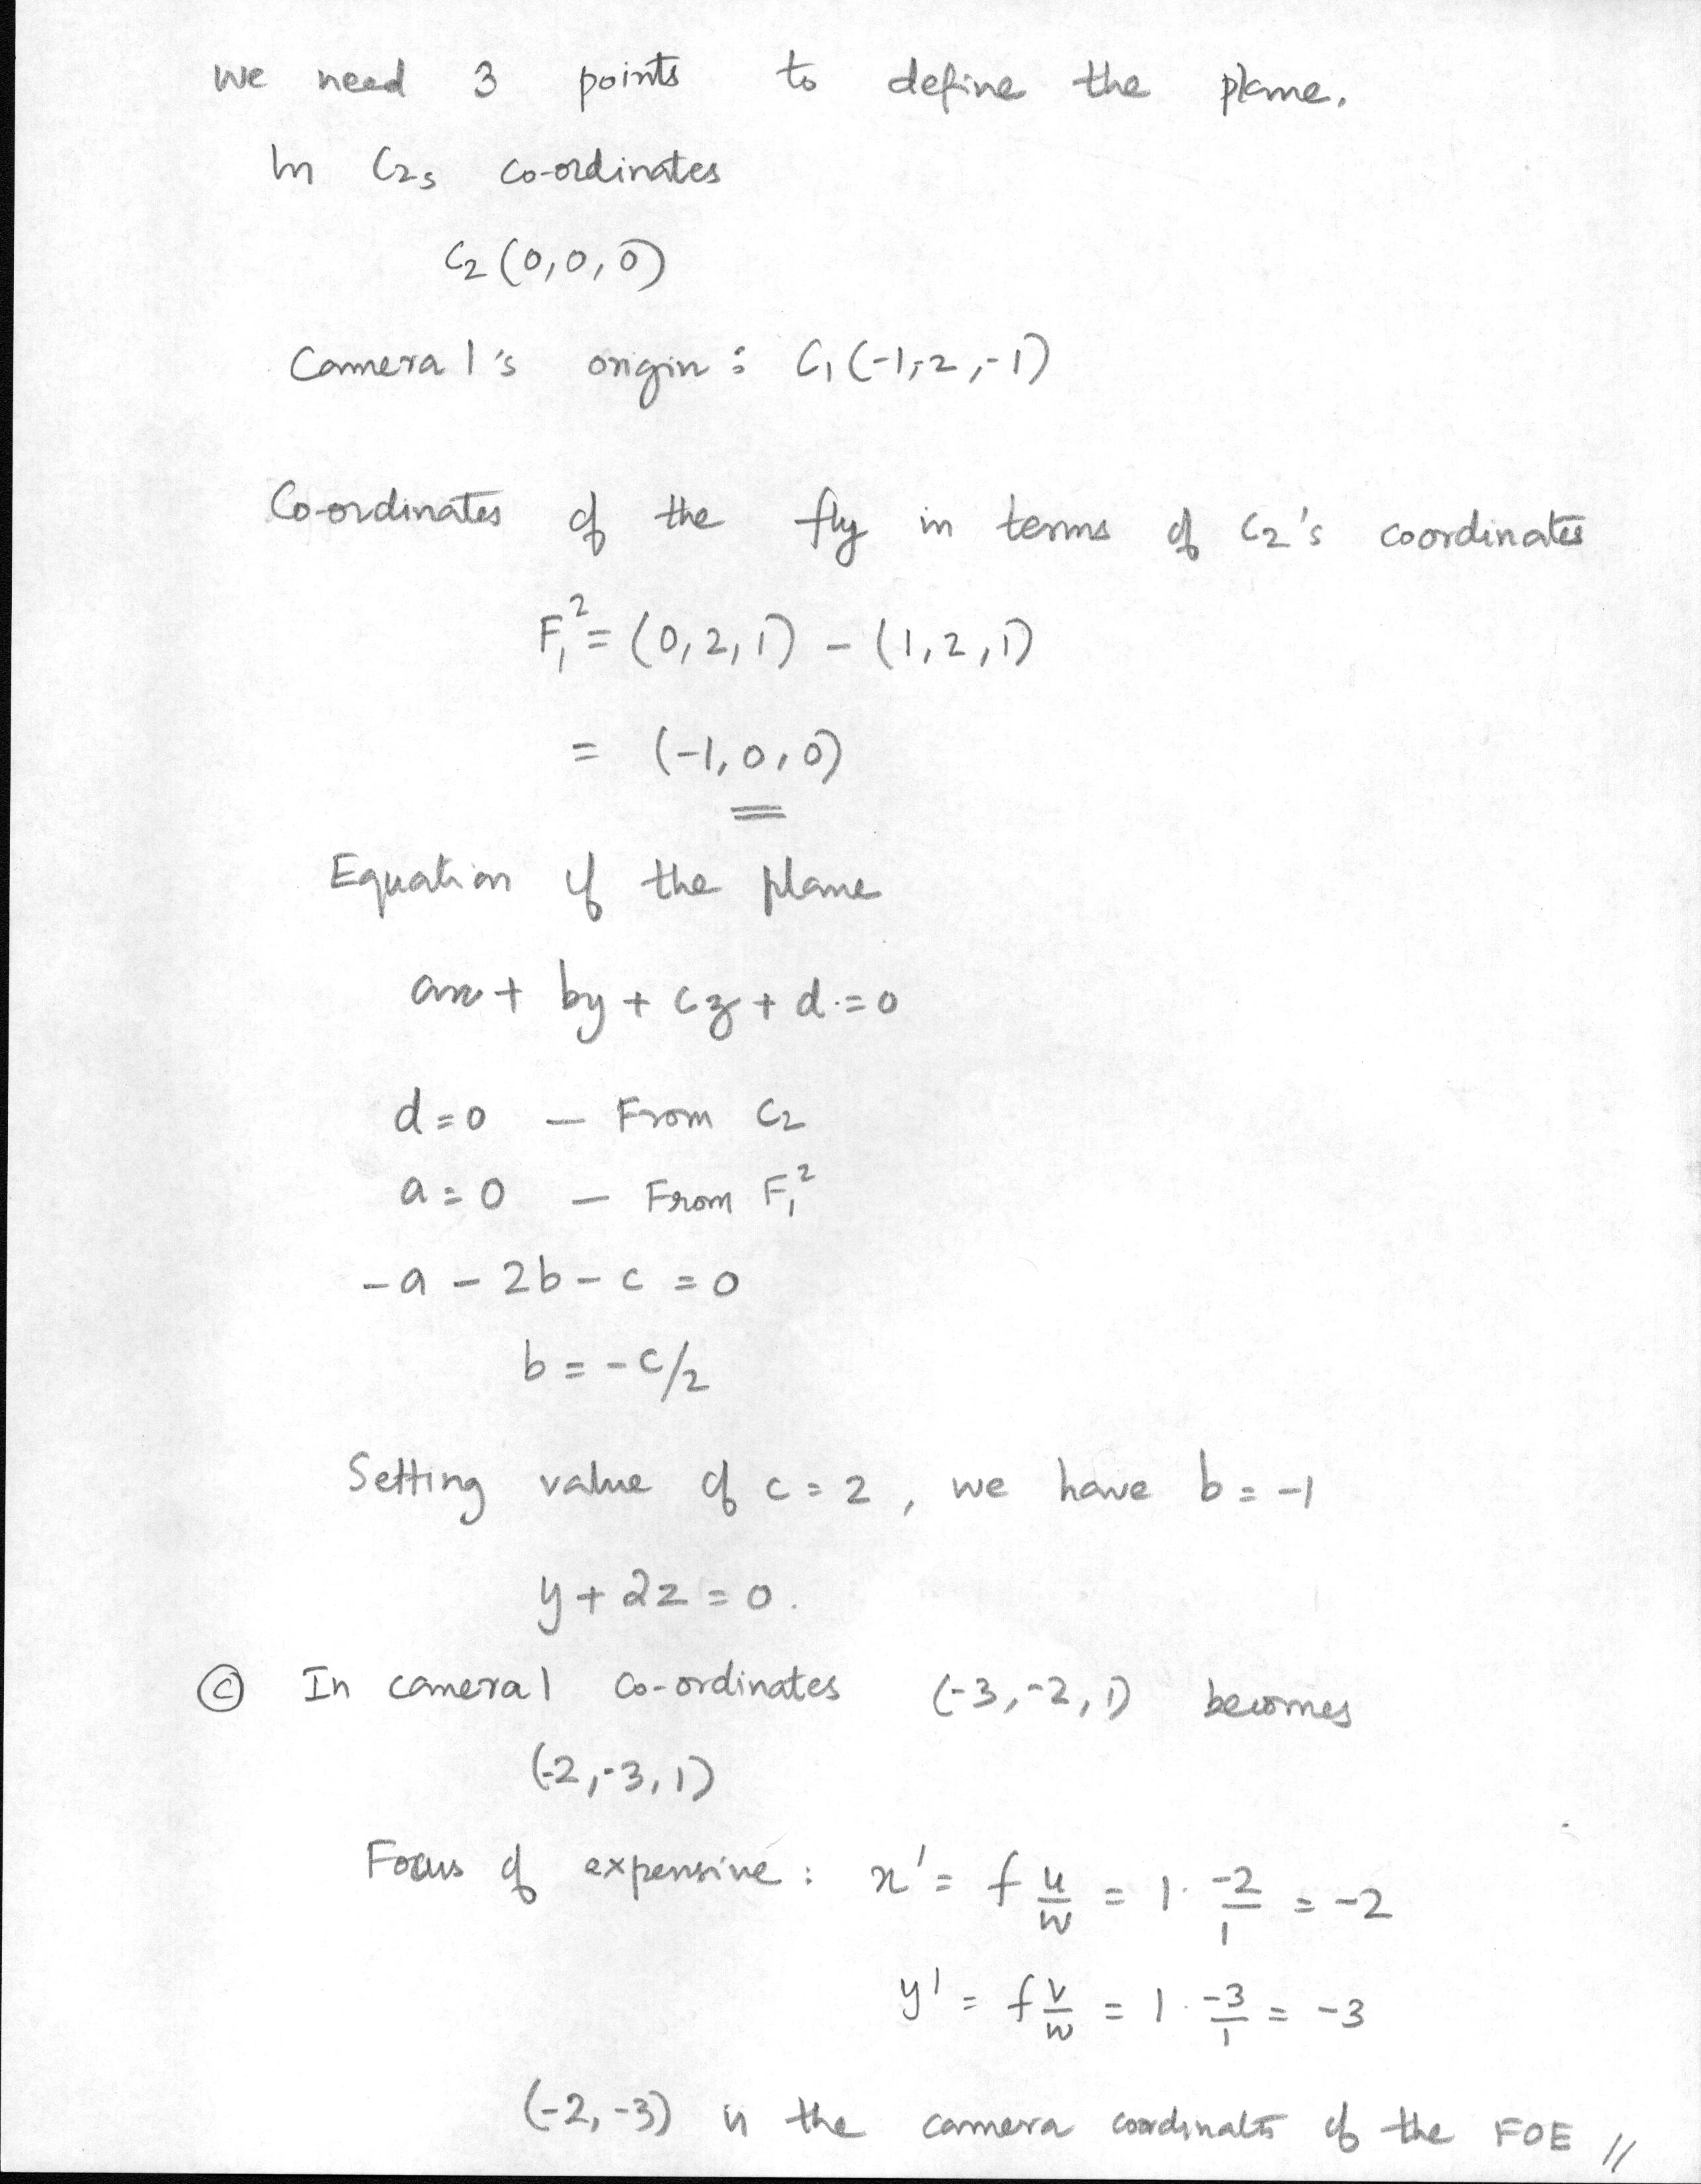
\includegraphics[width=15cm]{5.jpg}
\end{figure}

\begin{figure}
\section*{Question 8}  
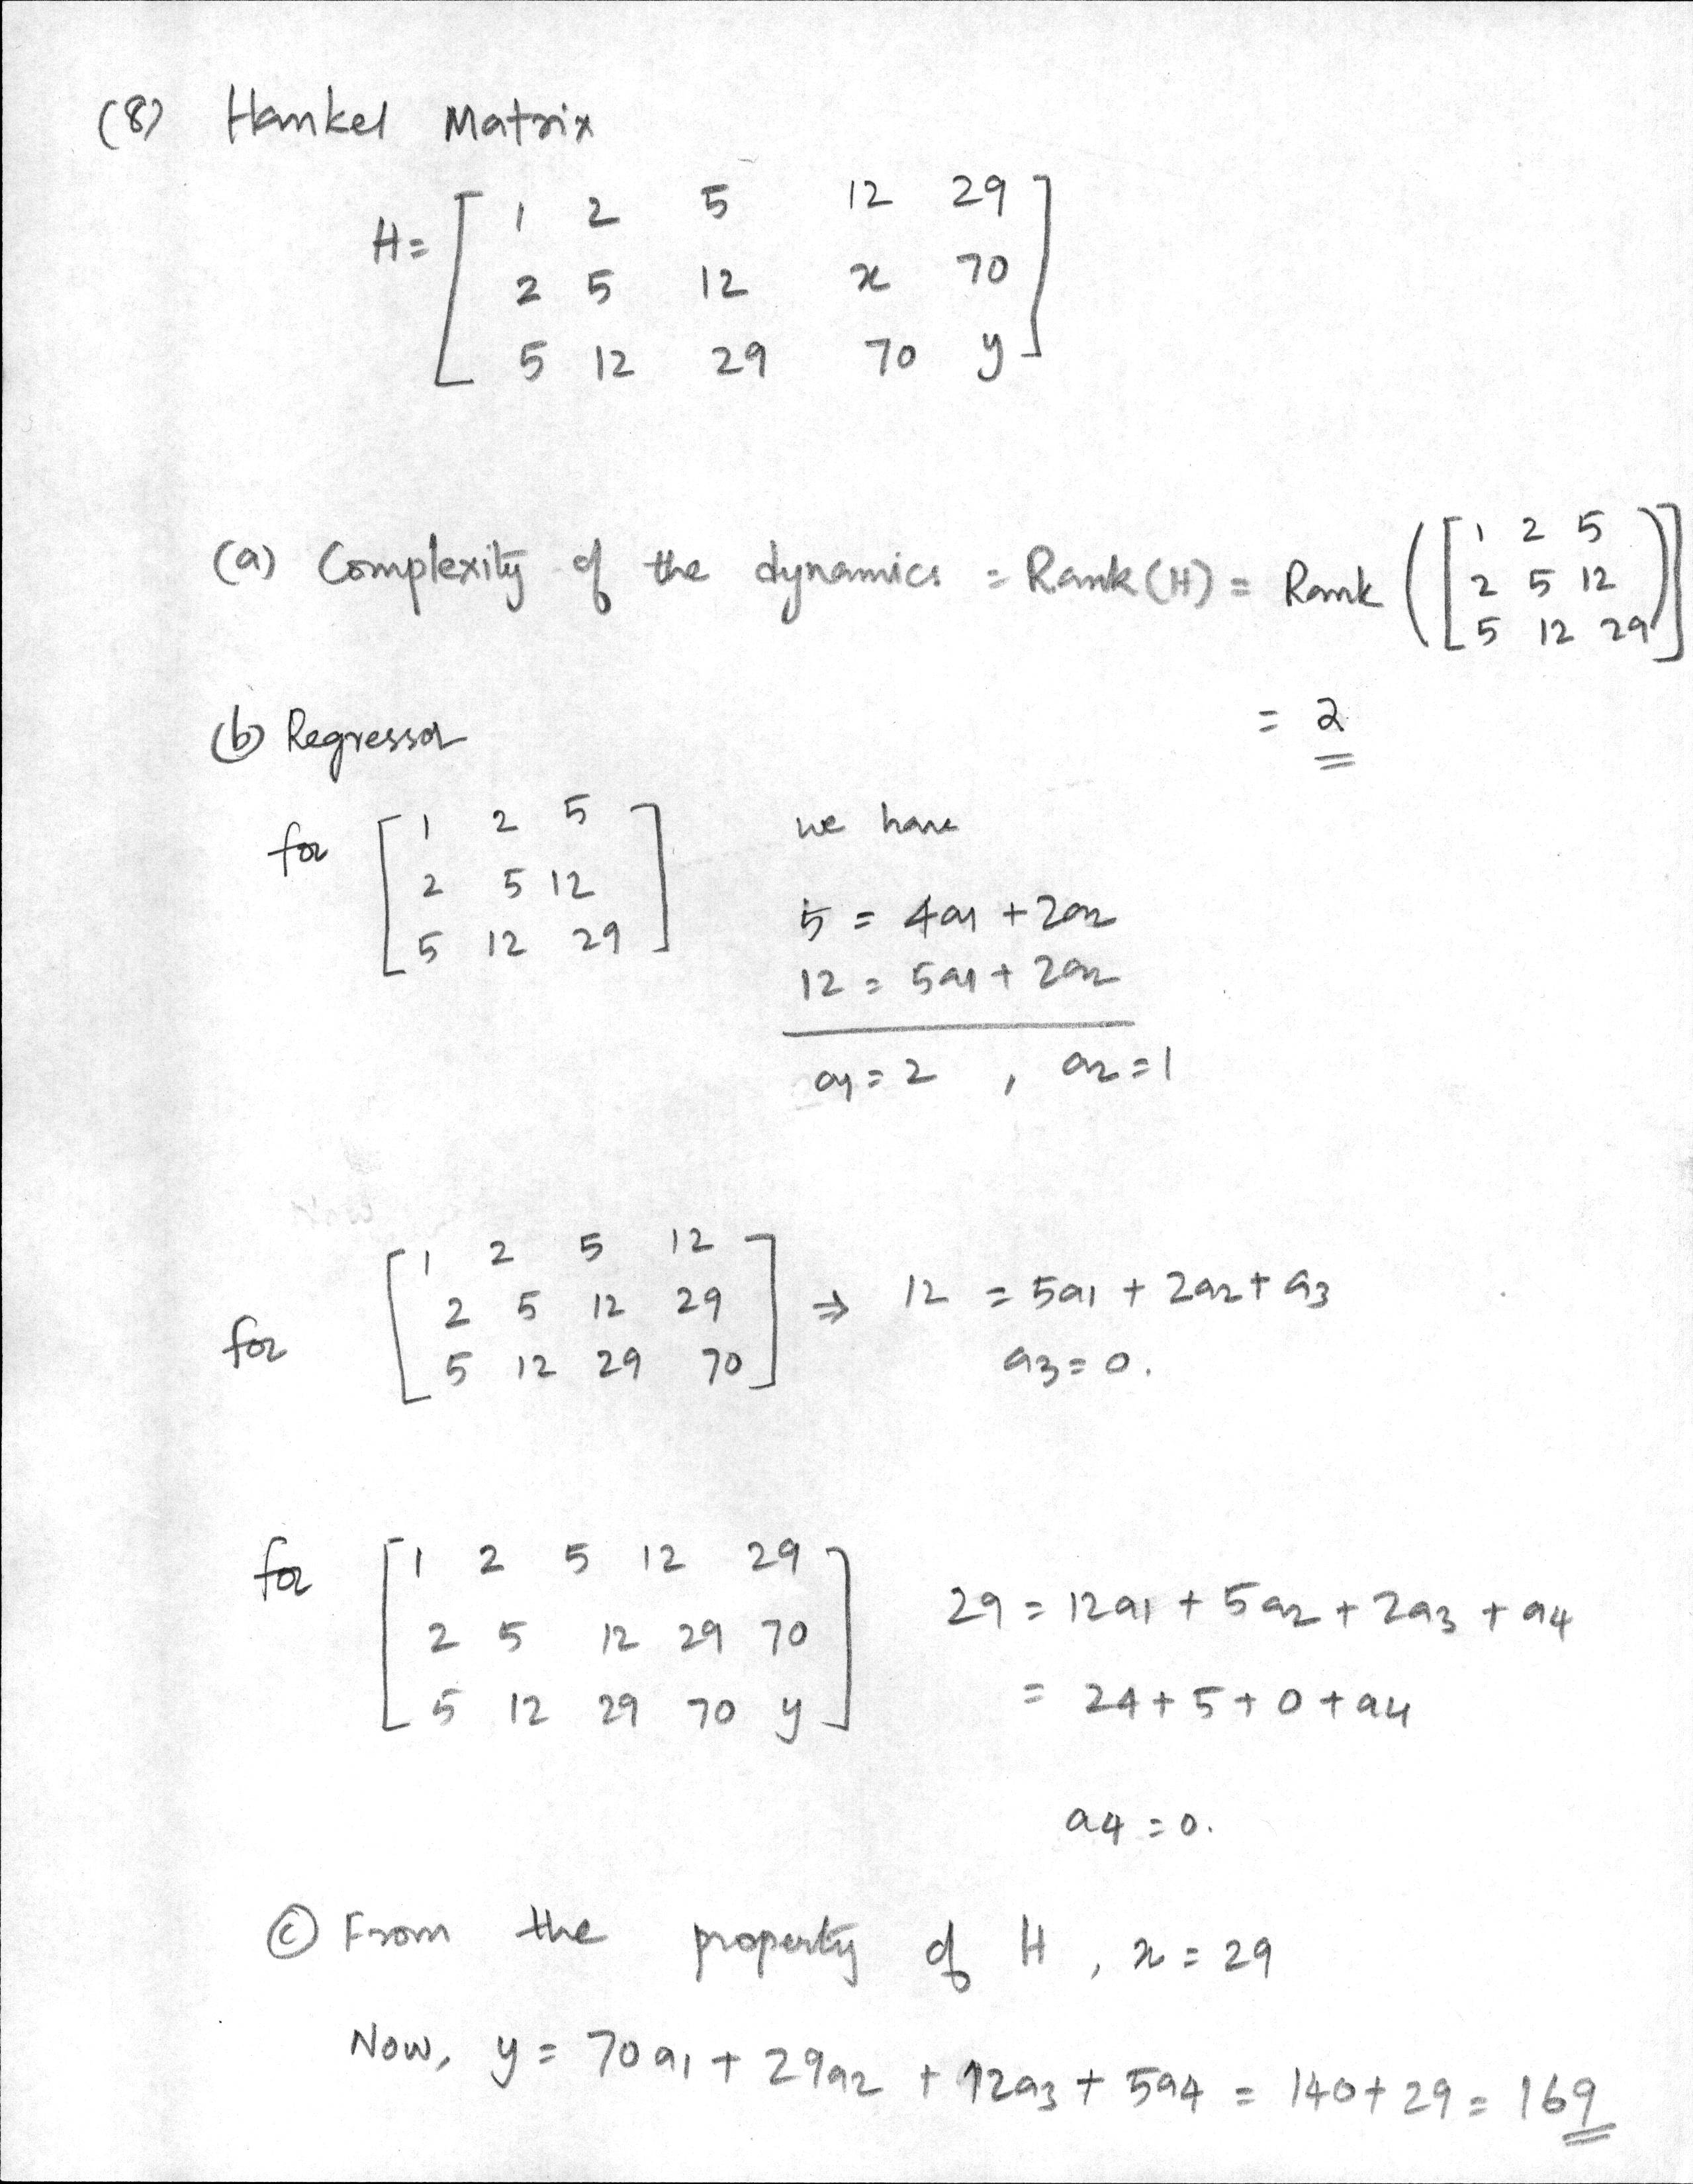
\includegraphics[width=15cm]{6.jpg}
\end{figure}


\end{document}



